%===================================== CHAP 6 =================================
\chapter{Experimental Setup}



\section{Data}
For this thesis we have mainly used FPL data provided by fantasyoverlord.com. Fantasy overlord contains detailed gameweek data for both the 2016/2017- and the 2017/2018 season. Further, clubelo.com has been used in order to obtain ELO values for each Premier League team. In addition, Sportradar has provided odds and probabilities for the fixtures of the 2017/2018 season. 
\newpar
The model presented in chapter \ref{chapter_model_formulation} has been run for the first 35 gameweeks of the 2017/2018 season. Ideally, the model should be run for the entire season. However, due to the deadline of the thesis this was not possible. 

\subsection{Processing of player data}
\subsubsection{Injuries and suspensions}
Once a player is listed as injured and thus unavailable for the upcoming gameweek, it is reasonable to set his expected points to zero. In order to account for injury status, we created a matrix of 0's and 1's. Fit players are assigned with a value of 1, while injured players are assigned with a value of 0. By multiplying each player's expected points by this injury matrix, injured players' expected points are automatically set to zero. As it is difficult to decide exactly when an injured player will be fit again, it is assumed in the solution approach that once a player is listed as injured, he will be unavailable for the upcoming three gameweeks. However, the injury list is updated for each gameweek, hence a player's injury status might change after a gameweek has been played. During the season we have collected injury data from fantasypremierleague.com ahead of each gameweek. Players that were listed with a 0\% probability of playing were listed as injured for the upcoming gameweek. 
\newpar
In addition, the model accounts for suspensions when optimizing the team for a gameweek. A player may be suspended for up to three games when receiving a red card, depending on whether it was a direct red card or not. Further, a player is subject to a match ban if he receives his 5th, 10th or 15th yellow card of the season. In addition, a player can be suspended by the English Football Association if he is found guilty of unsportsmanlike conduct. As for the injuries, a player that is suspended is rewarded with an expected points of 0 in the gameweeks of his suspensions. 

\subsubsection{Promoted teams}
Gathering data for newly promoted teams is rather difficult, as this data is not easy obtainable. In addition, it requires a lot of computational work in order to compare performances in the English Championship to the Premier League. Due to these difficulties, some simplifications are made. In general, players on newly promoted teams are not considered in the first gameweek of the 2017/2018 season. However, if a player was transferred to a promoted team ahead of the season, and he played in the Premier League in the previous season, the player would then be considered from the start of the season. It is worth noticing that the newly promoted teams are partly considered in the first gameweek when using the average method. This is solved by using the ELO system. 
\subsubsection{Players transferred ahead of 2017/2018 season}
A question that arise with the international transfer window, is how new players is going to perform in another league in a different country. Forecasts of these players performance could be obtained by studying their performance from previous seasons in their respective leagues and hence somehow compare a performance in a different league with a performance in Premier League. However, it is very difficult to compare one league to another. Further, it must be done for several leagues, for instance the Spanish La Liga, the Italian Serie A, the German Bundesliga, the Dutch Eredivisie etc. For simplicity, this type of work is not considered in this thesis.
\newpar
In this project it is assumed that the creators of Fantasy Premier League have assigned new players with a price that is perfectly mirrored by their expected performance. Thus, one can compare the new players with existing FPL players of the same price. For instance, if a new midfielder is listed with a price of 9, it is assumed that this player will have the same expected performance as other midfielders listed with the same price.
\subsubsection{Irregular gameweeks}
In general, every gameweek consists of 10 fixtures featuring every team once. However, due to matches in the national and international cups, some of the Premier League matches are postponed or played ahead of the original date. This implies that some of the gameweeks do not consist of exactly 10 fixtures, but perhaps 8 or 12 for instance. Thus, in these gameweeks some players may be featured twice, gaining points for both matches. Similarly, some players will not be feautered in other gameweeks, these gameweeks are hereby refered to as \textit{blanks}.


\section{Setting Parameters}
veldig viktig diskusjon: 
at vi har forstått at det er feil å sette høye penalties, men at vi er ute etter å få en modell som presterer bra. 
\subsection{Average}
In this thesis, the relative team strength factor are calculated according to the Elo values provided by clubelo.com. As the Elo values are updated for every gameweek, each Premier League team is assigned with 38 different Elo values, depending on the results in their previous games. An overview of the Elo values is attached in the appendix. 
\newpar
Table \ref{Field advantage} provides the calculated values for field advantages for the past five Premier League seasons. As can easily be observed, the field advantages seems to be somewhat constant, ranging from 1.105 to 1.149. Hence, simply taking the average over the past five years seems to yield an appropriate field advantage factor. 

\begin{table}[H]
\centering
\caption{Field advantages for previous 5 seasons}
\label{Field advantage}
\begin{tabular}{|l|l|l|l|l|l|l|}
\hline
          & 16-17    & 15-16    & 14-15    & 13-14    & 12 13 & \textbf{Average}   \\
          \hline
        
Home field advantage & 1.141 & 1.105 & 1.149 & 1.137 & 1.114 & \textbf{1.129} \\
\hline
Away field advantage & 0.859 & 0.895 & 0.851 & 0.863 & 0.886 & \textbf{0.871} \\
\hline
\end{tabular}
\end{table}

As for the point streak factor, the variables X and Y has to be decided. As goalkeepers and defenders receive 4 points for keeping a clean sheet, all players get 3 points for an assist and midfielders and forwards get 5 and 4 points respectively for scoring a goal, the X variable should be set according to these numbers. Further, as a player gets 2 points for playing more than 60 minutes, it is appropriate to let the X variable take a value of 5. Hence, if a player has an assist or scores a goal and in addition plays 60 minutes or more that player will receive enough points to be on a positive point streak given that he did not receive a yellow or red card. As for the Y variable, a player that does not contribute with neither a goal, assist nor a clean sheet is awarded maximum 2 points. Thus, it is reasonable to set the Y to equal 2 points. 
\subsubsection{Determining optimal forecasting horizon, optimization horizon and penalty term}

In a case with perfect information available, the optimal optimization horizon is the complete season of 38 gameweeks. Furthermore, the penalty term would be 4, equal as in the real case. However, we do not operate within the domain of perfect information, so these parameter settings are not guaranteed optimal. In addition, it is important to decide how many matches to look back in the past when calculating the forecasts based on average performance in previous games.
\newpar 
In order to set the values of the parameters in a smart way, a number of different combinations of the three parameters are run on the 2016/2017 season. Figure \ref{Parameter_choice} displays how the mean value of points for the entire 2016/2017 season changes with different forecasting horizons, optimization horizons and penalty terms. 

\begin{figure}[H]
    \centering
    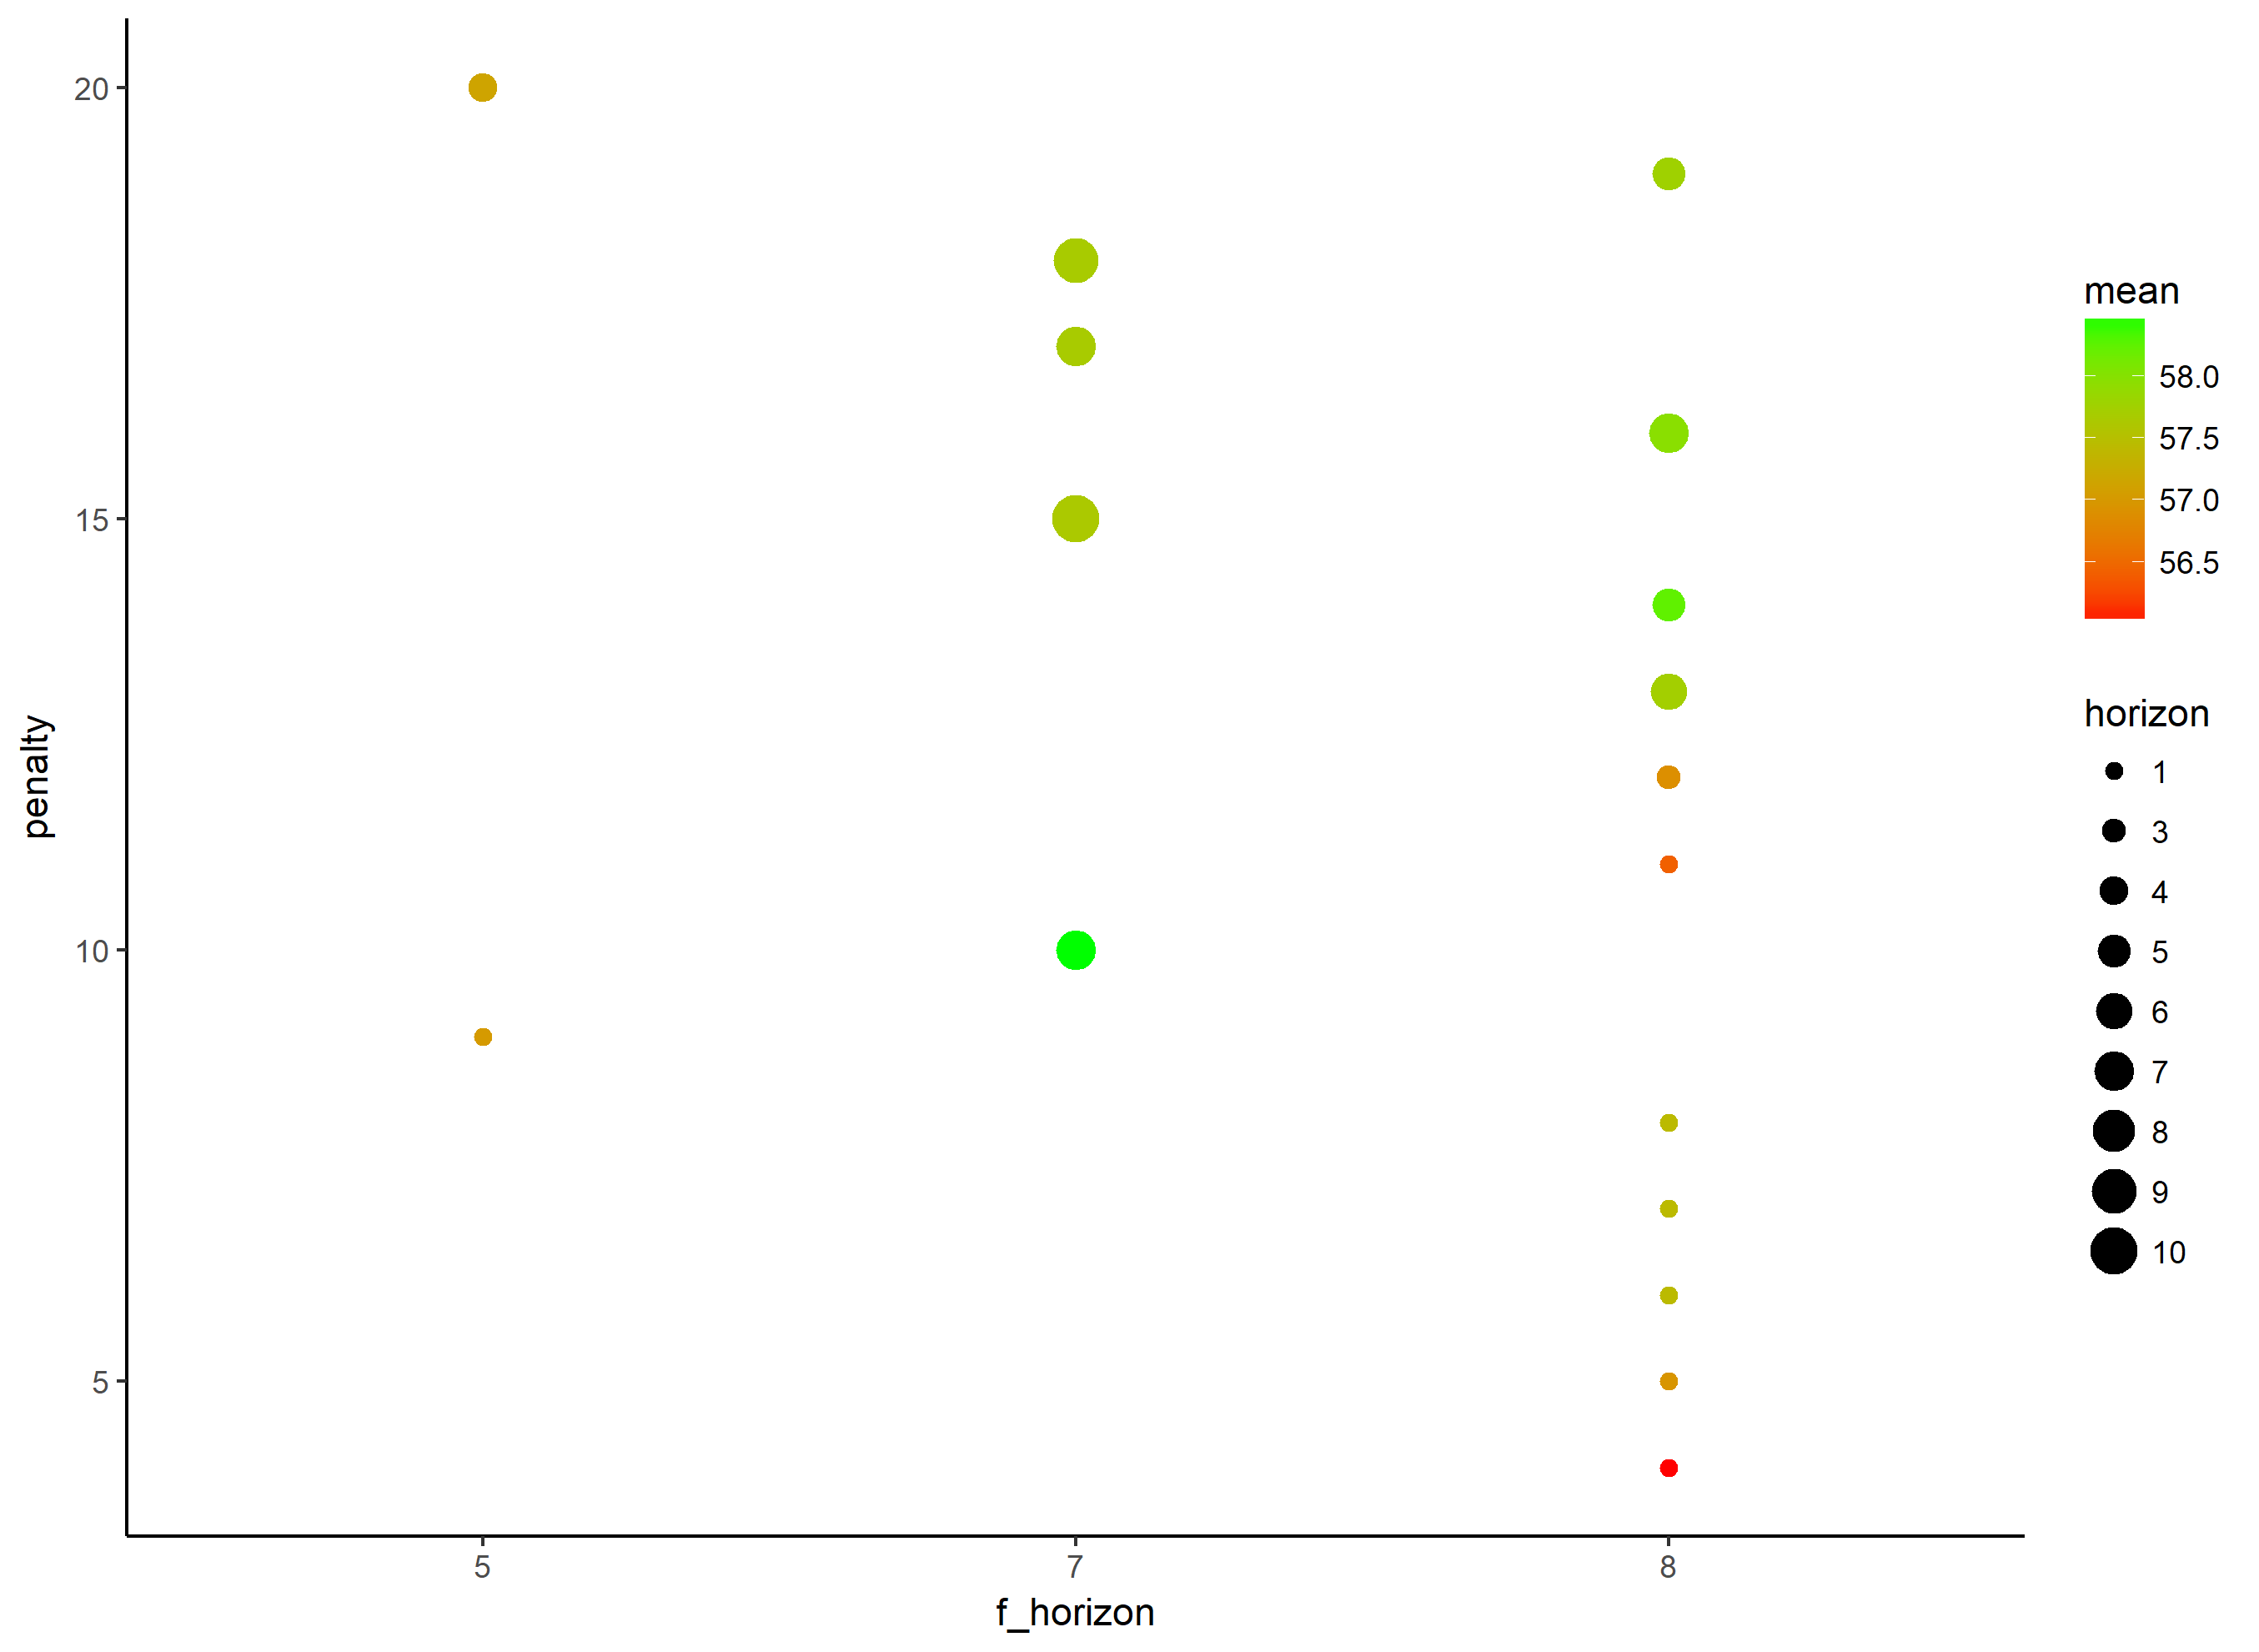
\includegraphics[scale=0.55]{fig/paramter_choice.png}
    \caption{Performance with different transfer penalties and forecast horizons}
\label{Parameter_choice}    
\end{figure}

In general, one can see that low transfer penalties combined with a high forecast horizon yield the poorest results. Furthermore, it seems like choosing 7 or 8 as the forecast horizon is the wiser choice. In addition, the transfer penalty should be set to a value above 10. Based on figure \ref{Parameter_choice}, a combination found in the center appears to be optimal, and the values $h = 6$, $f = 7$ and $p = 11$ are chosen. Also, a combination of $h = 4$, $f = 8$ and $p = 14$ yield good results. 
\newpar
As only data for the FPL 2015/2016 season is used, we were unable to predict points for the first gameweek of 2016/2017. Hence, when finding the optimal forecasting horizon the first gameweek is not considered. As for the forecast horizon of 8 weeks, we only consider the matches after gameweek 8 has been played. Hence, we get an opportunity of initially selecting the players that have performed best over the 8 first gameweeks. This is a great drawback when chosing the optimal forecast horizon. Intuitively, the results will be better as the forecast horizon increases, as one get the opportunity of initially selecting players that have proven to perform well. Hence, the mean of the teams performance is likely to rice above the mean if we started in gameweek 1. Therefore, based on the results from table \ref{Parameter_choice} we find it proper to choose the best mean with a smaller f-value, as this includes more gameweeks.  

\subsection{Linear Regression}
\subsection{Odds}
In order to obtain necessary data, we have cooperated with Sportradar, a Norwegian company providing data for bookmakers. Sportradar delivers odds and probabilities of several sports events, including English Premier League. They have provided us with all the necessary probabilities, including result outcomes for each Premier League match as well as individual player probabilities. These data made all the computational work a lot easier, as Sportradar exported structured excel files containing all the necessary data. 
\newpar
As odds are primarily available for fixtures in the near future, in general for the upcoming gameweek, the suggested solution approach using odds is rather limited. Hence, the horizon on the optimization model is forced to be one gameweek. Compared to the other suggested methods, this is considered a great drawback.
\section{Game Chips}
\section{Risk/Variance}

